\documentclass{ximera}
\graphicspath{  %% When looking for images,
{./}            %% look here first,
{./pictures/}   %% then look for a pictures folder,
{../pictures/}  %% which may be a directory up.
{../../pictures/}  %% which may be a directory up.
{../../../pictures/}  %% which may be a directory up.
{../../../../pictures/}  %% which may be a directory up.
}

\usepackage{listings}
%\usepackage{circuitikz}
\usepackage{xcolor}
\usepackage{amsmath,amsthm}
\usepackage{subcaption}
\usepackage{graphicx}
\usepackage{tikz}
%\usepackage{tikz-3dplot}
\usepackage{amsfonts}
%\usepackage{mdframed} % For framing content
%\usepackage{tikz-cd}

  \renewcommand{\vector}[1]{\left\langle #1\right\rangle}
  \newcommand{\arrowvec}[1]{{\overset{\rightharpoonup}{#1}}}
  \newcommand{\ro}{\texttt{R}}%% row operation
  \newcommand{\dotp}{\bullet}%% dot product
  \renewcommand{\l}{\ell}
  \let\defaultAnswerFormat\answerFormatBoxed
  \usetikzlibrary{calc,bending}
  \tikzset{>=stealth}
  




%make a maroon color
\definecolor{maroon}{RGB}{128,0,0}
%make a dark blue color
\definecolor{darkblue}{RGB}{0,0,139}
%define the color fourier0 to be the maroon color
\definecolor{fourier0}{RGB}{128,0,0}
%define the color fourier1 to be the dark blue color
\definecolor{fourier1}{RGB}{0,0,139}
%define the color fourier 1t to be the light blue color
\definecolor{fourier1t}{RGB}{173,216,230}
%define the color fourier2 to be the dark green color
\definecolor{fourier2}{RGB}{0,100,0}
%define teh color fourier2t to be the light green color
\definecolor{fourier2t}{RGB}{144,238,144}
%define the color fourier3 to be the dark purple color
\definecolor{fourier3}{RGB}{128,0,128}
%define the color fourier3t to be the light purple color
\definecolor{fourier3t}{RGB}{221,160,221}
%define the color fourier0t to be the red color
\definecolor{fourier0t}{RGB}{255,0,0}
%define the color fourier4 to be the orange color
\definecolor{fourier4}{RGB}{255,165,0}
%define the color fourier4t to be the darker orange color
\definecolor{fourier4t}{RGB}{255,215,0}
%define the color fourier5 to be the yellow color
\definecolor{fourier5}{RGB}{255,255,0}
%define the color fourier5t to be the darker yellow color
\definecolor{fourier5t}{RGB}{255,255,100}
%define the color fourier6 to be the green color
\definecolor{fourier6}{RGB}{0,128,0}
%define the color fourier6t to be the darker green color
\definecolor{fourier6t}{RGB}{0,255,0}

%New commands for this doc for errors in copying
\newcommand{\eigenvar}{\lambda}
%\newcommand{\vect}[1]{\mathbf{#1}}
\renewcommand{\th}{^{\text{th}}}
\newcommand{\st}{^{\text{st}}}
\newcommand{\nd}{^{\text{nd}}}
\newcommand{\rd}{^{\text{rd}}}
\newcommand{\paren}[1]{\left(#1\right)}
\newcommand{\abs}[1]{\left|#1\right|}
\newcommand{\R}{\mathbb{R}}
\newcommand{\C}{\mathbb{C}}
\newcommand{\Hilb}{\mathbb{H}}
\newcommand{\qq}[1]{\text{#1}}
\newcommand{\Z}{\mathbb{Z}}
\newcommand{\N}{\mathbb{N}}
\newcommand{\q}[1]{\text{``#1''}}
%\newcommand{\mat}[1]{\begin{bmatrix}#1\end{bmatrix}}
\newcommand{\rref}{\text{reduced row echelon form}}
\newcommand{\ef}{\text{echelon form}}
\newcommand{\ohm}{\Omega}
\newcommand{\volt}{\text{V}}
\newcommand{\amp}{\text{A}}
\newcommand{\Seq}{\textbf{Seq}}
\newcommand{\Poly}{\textbf{P}}
\renewcommand{\quad}{\text{    }}
\newcommand{\roweq}{\simeq}
\newcommand{\rowop}{\simeq}
\newcommand{\rowswap}{\leftrightarrow}
\newcommand{\Mat}{\textbf{M}}
\newcommand{\Func}{\textbf{Func}}
\newcommand{\Hw}{\textbf{Hamming weight}}
\newcommand{\Hd}{\textbf{Hamming distance}}
\newcommand{\rank}{\text{rank}}
\newcommand{\longvect}[1]{\overrightarrow{#1}}
% Define the circled command
\newcommand{\circled}[1]{%
  \tikz[baseline=(char.base)]{
    \node[shape=circle,draw,inner sep=2pt,red,fill=red!20,text=black] (char) {#1};}%
}

% Define custom command \strikeh that just puts red text on the 2nd argument
\newcommand{\strikeh}[2]{\textcolor{red}{#2}}

% Define custom command \strikev that just puts red text on the 2nd argument
\newcommand{\strikev}[2]{\textcolor{red}{#2}}

%more new commands for this doc for errors in copying
\newcommand{\SI}{\text{SI}}
\newcommand{\kg}{\text{kg}}
\newcommand{\m}{\text{m}}
\newcommand{\s}{\text{s}}
\newcommand{\norm}[1]{\left\|#1\right\|}
\newcommand{\col}{\text{col}}
\newcommand{\sspan}{\text{span}}
\newcommand{\proj}{\text{proj}}
\newcommand{\set}[1]{\left\{#1\right\}}
\newcommand{\degC}{^\circ\text{C}}
\newcommand{\centroid}[1]{\overline{#1}}
\newcommand{\dotprod}{\boldsymbol{\cdot}}
%\newcommand{\coord}[1]{\begin{bmatrix}#1\end{bmatrix}}
\newcommand{\iprod}[1]{\langle #1 \rangle}
\newcommand{\adjoint}{^{*}}
\newcommand{\conjugate}[1]{\overline{#1}}
\newcommand{\eigenvarA}{\lambda}
\newcommand{\eigenvarB}{\mu}
\newcommand{\orth}{\perp}
\newcommand{\bigbracket}[1]{\left[#1\right]}
\newcommand{\textiff}{\text{ if and only if }}
\newcommand{\adj}{\text{adj}}
\newcommand{\ijth}{\emph{ij}^\text{th}}
\newcommand{\minor}[2]{M_{#2}}
\newcommand{\cofactor}{\text{C}}
\newcommand{\shift}{\textbf{shift}}
\newcommand{\startmat}[1]{
  \left[\begin{array}{#1}
}
\newcommand{\stopmat}{\end{array}\right]}
%a command to give a name to explorations and hints and theorems
\newcommand{\name}[1]{\begin{centering}\textbf{#1}\end{centering}}
\newcommand{\vect}[1]{\vec{#1}}
\newcommand{\dfn}[1]{\textbf{#1}}
\newcommand{\transpose}{\mathsf{T}}
\newcommand{\mtlb}[2][black]{\texttt{\textcolor{#1}{#2}}}
\newcommand{\RR}{\mathbb{R}} % Real numbers
\newcommand{\id}{\text{id}}
\newcommand{\coord}[1]{\langle#1\rangle}
\newcommand{\RREF}{\text{RREF}}
\newcommand{\Null}{\text{Null}}
\newcommand{\Nullity}{\text{Nullity}}
\newcommand{\Rank}{\text{Rank}}
\newcommand{\Col}{\text{Col}}
\newcommand{\Ef}{\text{EF}}
\newcommand{\boxprod}[3]{\abs{(#1\times#2)\cdot#3}}

\author{Zack Reed}
%borrowed from selinger linear algebra
\title{Singular Value Decomposition (SVD)}
\begin{document}
\begin{abstract}

    In this learning activity, you will be 
\end{abstract}
\maketitle

\section*{Introduction}
In machine learning (ML), some of the most important linear algebra concepts are the \textbf{singular value decomposition (SVD)} and \textbf{principal component analysis (PCA)}. With all the raw data collected, how can we discover structures? For example, with the interest rates of the last 6 days, can we understand its composition to spot trends?

This becomes even harder for high-dimensional raw data. It is like finding a needle in a haystack. SVD allows us to extract and untangle information. In this article, we will detail SVD and PCA. We assume you have basic linear algebra knowledge, including rank and eigenvectors. If you experience difficulties in reading this article, I will suggest refreshing those concepts first. At the end of the article, we will answer some questions in the interest rate example above. This article also contains optional sections. Feel free to skip them according to your interest level.

\section*{Misconceptions (optional for beginners)}
Some common questions that non-beginners may ask include whether PCA is only for dimension reduction. PCA reduces dimension but is far more than that. As described in Wikipedia:

\begin{quote}
Principal component analysis (PCA) is a statistical procedure that uses an orthogonal transformation to convert a set of observations of possibly correlated variables (entities each of which takes on various numerical values) into a set of values of linearly uncorrelated variables called principal components.
\end{quote}

From a simplified perspective, PCA transforms data linearly into new properties that are uncorrelated. For ML, positioning PCA as feature extraction may allow us to explore its potential better than just dimension reduction.

\section{SVD and PCA Differences}
SVD decomposes a matrix into special matrices that are easy to manipulate and analyze. PCA focuses on the most significant components. SVD allows for finding PCA by truncating less important basis vectors in the original SVD matrix.

\section{Matrix Diagonalization}
In the article on eigenvalue and eigenvectors, we describe a method to decompose an \(n \times n\) square matrix \(A\) into:

\[
A = PDP^{-1}
\]

where \(D\) is a diagonal matrix containing eigenvalues of \(A\).

\section{Singular Vectors \& Singular Values}
For any \(m \times n\) matrix \(A\), consider \(AA^\top\) and \(A^\top A\):

\begin{itemize}
    \item symmetrical,
    \item square,
    \item at least positive semidefinite (eigenvalues are zero or positive),
    \item both matrices have the same positive eigenvalues, and
    \item both have the same rank \(r\) as \(A\).
\end{itemize}

These matrices, common in ML, allow us to find orthonormal eigenvectors.

Let’s introduce some terms. The eigenvectors of \(AA^\top\) are denoted by \(u_i\) and of \(A^\top A\) by \(v_i\), known as the \textbf{singular vectors} of \(A\). Their square roots are called \textbf{singular values}.

\section{SVD}
Any matrix \(A\) can be factorized as:

\[
A = U \Sigma V^\top
\]

where \(U\) and \(V\) are orthogonal matrices and \(\Sigma\) is a diagonal matrix with elements equal to the square root of the positive eigenvalues of \(AA^\top\) or \(A^\top A\).

\[
A = U \begin{bmatrix} \sigma_1 & 0 & \cdots \\ 0 & \sigma_2 & \cdots \\ \vdots & \vdots & \ddots \end{bmatrix} V^\top
\]

The columns of \(U\) are called the left singular vectors, and those of \(V\) are the right singular vectors.

\section{Example}
Consider an example of a simple \(2 \times 2\) matrix. We calculate:

\[
A = \begin{bmatrix} 3 & 1 \\ 1 & 3 \end{bmatrix}
\]

The singular values are \(\sigma_1 = 5\) and \(\sigma_2 = 3\). Thus, the SVD composition is:

\[
A = U \Sigma V^\top
\]

\section{Recap of SVD}
The SVD decomposition of \(A\) can be summarized as:

\[
A = U \Sigma V^\top
\]

where

\[
U^\top U = I \quad \text{and} \quad V^\top V = I
\]

\section{Moore-Penrose Pseudoinverse}
To find the best-fit solution, we compute a pseudoinverse of \(A\) that minimizes the least square error:

\[
A^+ = V \Sigma^+ U^\top
\]

\section{Variance \& Covariance}
The sample variance is defined as:

\[
s^2 = \frac{1}{n-1} \sum_{i=1}^n (x_i - \bar{x})^2
\]

The covariance matrix \(\Sigma\) captures variance along the diagonal elements and covariance between variables in the non-diagonal elements.

\section{Covariance Matrix \& SVD}
The SVD decomposition of a covariance matrix reveals the principal components of data. The total variance of the data equals the trace of the covariance matrix, which is the sum of the squares of singular values.

\section{Principal Component Analysis (PCA)}
Technically, SVD extracts data in the directions with the highest variances. PCA uses SVD for mapping data to principal components, allowing dimensionality reduction by ignoring less significant terms.

One of the early and natural ideas in software development for scientific computation was the idea of packaging linear algebra software around robust implementations of matrix factorizations, divested from specific applications. This enabled durable linear algebra tools like LAPACK to be developed with a stable interface, usable across numerous application domains. Commercial software like Matlab™, as well as open-source software like Octave, numpy, and scipy, all take full advantage of these developments. What does this mean for you as an aspiring data scientist? When you are faced with a specific computational task, if you are able to reformulate your task using off-the-shelf implementations of matrix factorizations, then you might already be halfway to finishing your task.

You already know about some matrix factorizations. In your introductory linear algebra prerequisites, you learned about eigenvalues and eigenvectors. The computation of eigenvalues and eigenvectors is indeed the computation of a matrix factorization. This factorization is called a diagonalization or an eigenvalue decomposition of an \( n \times n \) matrix \( A \) and it takes the form

\[
A = X D X^{-1}
\]

where \( D \) is a diagonal matrix and \( X \) is an invertible matrix, both of the same size as \( A \). The eigenvalues of \( A \) are found in the diagonal entries of \( D \) and the eigenvectors are columns of \( X \), as can be seen by rewriting the factorization as

\[
A X = X D.
\]

The importance of eigenvalues in varied applications is usually highlighted well in a first linear algebra course.

Another important factorization is the SVD, or the singular value decomposition, which often does not get the emphasis it deserves in lower-division courses. In some ways, the SVD is even more important than diagonalization. This is because not all matrices have a diagonalization. In contrast, using basic real analysis results, one can prove that any matrix has an SVD. We shall see that from an SVD, one can read off the important properties of a matrix and easily construct compressed approximations of the matrix.

\section{Definition of SVD}

The SVD is a factorization of an \( m \times n \) matrix \( A \) of the form

\[
A = U \Sigma V^*
\]

where \( \Sigma \) is an \( m \times n \) diagonal matrix, and \( U \) and \( V \) are unitary matrices of size \( m \times m \) and \( n \times n \), respectively. (Recall that a square matrix \( Q \) is called unitary if its inverse equals \( Q^* \), the conjugate transpose of \( Q \).) The diagonal entries of \( \Sigma \) are non-negative, and positive ones are called the singular values of \( A \). It is a convention to list the singular values in non-increasing order along the diagonal. The columns of \( U \) and \( V \) are called the left and right singular vectors, respectively.

Here is how we compute SVD using MATLAB:

\begin{verbatim}
[U, S, V] = svd(rand(4, 5) + 1i * rand(4, 5));
U * U'  % U is unitary. Its columns are left singular vectors
V * V'  % Rows of V are right singular vectors
diag(S) % Only the diagonal entries of Sigma are returned in S
\end{verbatim}

\section{The Algebra of SVD}

An outer product of an \( x \in \mathbb{R}^m \) and \( y \in \mathbb{R}^n \) is the \( m \times n \) matrix \( x y^* \) (which, being the product of \( m \times 1 \) and \( 1 \times n \) matrices, is of shape \( m \times n \)). Reversing the order of \( x \) and \( y^* \) in the product, we get the familiar inner product, which is a \( 1 \times 1 \) matrix or a scalar.

Naming the columns of \( U \) and \( V \) as \( u_i \) and \( v_j \), we have

\[
A = U \Sigma V^* = \sum_{l=1}^{\min(m,n)} \sigma_l u_l v_l^*.
\]

Thus, the SVD can be viewed as a sum of unit-rank outer products. Each summand increases rank (if the corresponding singular value is nonzero) until the rank of \( A \) is reached. Let's see this in action for a small matrix in MATLAB.

\begin{verbatim}
a = rand(4, 5);
[U, S, V] = svd(a);
outer_product = U(:, 1) * V(1, :) * S(1, 1);
\end{verbatim}

\section{Low Rank Approximation}

A useful application of SVD is low-rank approximation. For an \( m \times n \) matrix \( A \) with singular values \( \sigma_j \), we can approximate \( A \) using the first few singular values:

\[
A_\ell = \sum_{j=1}^\ell \sigma_j u_j v_j^*.
\]

This is particularly useful for image compression. Here’s how to compute a low-rank approximation of an image using MATLAB:

\begin{verbatim}
img = imread('cats.png');
img = img(:,:,1); % Convert to grayscale
[U, S, V] = svd(double(img));
rank_20 = U(:, 1:20) * S(1:20, 1:20) * V(:, 1:20)';
imshow(uint8(rank_20), []);
\end{verbatim}

If you increase the rank, the approximation becomes closer to the original image. This technique not only reduces storage requirements but can also accelerate computations by reducing the dimensions of data.

\section{Further Applications}

The SVD is a fundamental tool for any data scientist. Whether it’s image compression, dimensionality reduction, or uncovering hidden structures in data, SVD provides a robust mathematical framework that continues to be valuable across many domains.

Returning to Theorem 2, notice that the theorem also gives one the ability to specify an error tolerance and let that dictate the choice of the rank \( \ell \). For example, if I do not want the error in my low-rank approximation to be more than some specific \( \epsilon \), then I need only choose \( \ell \) so that:

\[
\left( \sigma_{\ell+1}^2 + \cdots + \sigma_{r}^2 \right)^{1/2} \leq \epsilon.
\]

As an example, suppose I declare I want a low-rank approximation within the following relative error in Frobenius norm:

\begin{verbatim}
relative_error = 1.e-1;
\end{verbatim}

Then we can find the needed \( \ell \) using an aggregation and masking as follows:

\begin{verbatim}
s2 = s.^2;
total = sum(s2);
diff = sqrt((total - cumsum(s2)) / total);
l = find(diff < relative_error, 1);
l
\end{verbatim}

This will output:

\begin{verbatim}
l = 41
\end{verbatim}

Then, here is the needed low-rank approximation:

\begin{verbatim}
cl = U(:, 1:l) * diag(s(1:l)) * V(:, 1:l)';
\end{verbatim}

You can check that the error is indeed less than the prescribed error tolerance:

\begin{verbatim}
error = norm(c - cl, 'fro') / norm(c, 'fro');
error
\end{verbatim}

This returns:

\begin{verbatim}
error = 0.09942439
\end{verbatim}

As you can see, the low-rank approximation does give some image compression. The number of entries needed to store a rank \( \ell \) approximation \( cl \) of an \( m \times n \) matrix is \( m\ell + \ell + \ell n \):

\begin{verbatim}
entries_needed = size(U, 1) * l + l + l * size(V, 1);
entries_needed
\end{verbatim}

For instance, this might output:

\begin{verbatim}
entries_needed = 73759
\end{verbatim}

In contrast, to store the original image (single channel), we would need to minimally store \( mn \) numbers:

\begin{verbatim}
original_entries = size(c, 1) * size(c, 2);
original_entries
\end{verbatim}

Which might output:

\begin{verbatim}
original_entries = 788320
\end{verbatim}

Comparing the two outputs, we can certainly conclude that we have some compression. However, for image compression, there are better algorithms.

The utility of the low-rank approximation technique using the SVD is not really in image compression, but rather in other applications needing a condensed operator. Being a compressed approximation of an operator (i.e., a matrix) is much more than just a compressed visual image. For example, one can not only reduce the storage for a matrix but also reduce the time to apply the operator to a vector using a low-rank approximation. Because the SVD tells us the essentials of an operator in lower-dimensional spaces, it continues to find new applications in many modern emerging concepts, some of which we shall see in later lectures.
 
\begin{equation*}
    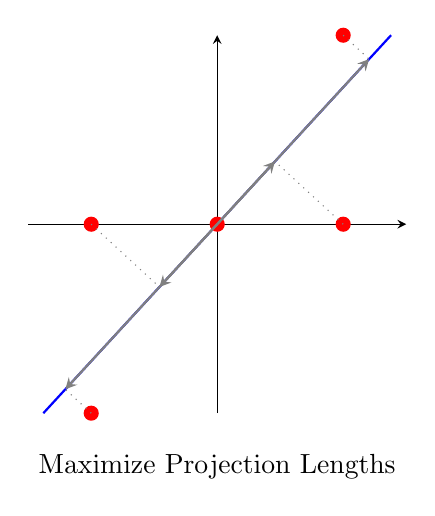
\begin{tikzpicture}[scale=0.8]
        \draw[thin,->] (-3,0) -- (3,0);
        \draw[thin,->] (0,-3) -- (0,3);
        \draw[thick,blue] (-3*0.92,-3) -- (3*0.92, 3);
        \fill[color=red] (0,0) circle (0.12);
        \fill[color=red] (2,0) circle (0.12);
        \fill[color=red] (2,3) circle (0.12);
        \fill[color=red] (-2,0) circle (0.12);
        \fill[color=red] (-2,-3) circle (0.12);
        \draw[thin, dotted,black!50] (2,0) -- (0.997*0.92,0.997);
        \draw[thin, dotted,black!50] (2,3) -- (2.621*0.92,2.621);
        \draw[thin, dotted,black!50] (-2,0) -- (-0.997*0.92,-0.997);
        \draw[thin, dotted,black!50] (-2,-3) -- (-2.621*0.92,-2.621);
        \draw[thick, ->,black!50] (0,0) -- (0.997*0.92,0.997);
        \draw[thick, ->,black!50] (0,0) -- (2.621*0.92,2.621);
        \draw[thick, ->,black!50] (0,0) -- (-0.997*0.92,-0.997);
        \draw[thick, ->,black!50] (0,0) -- (-2.621*0.92,-2.621);
        \path (0,-3.5) node[below] {Maximize Projection Lengths};
        %\path[black!70] (2,-2) node {\begin{tabular}{c}maximize\\projection\\lengths\\on subspace\end{tabular}};
      \end{tikzpicture}
    \hspace{1in}
    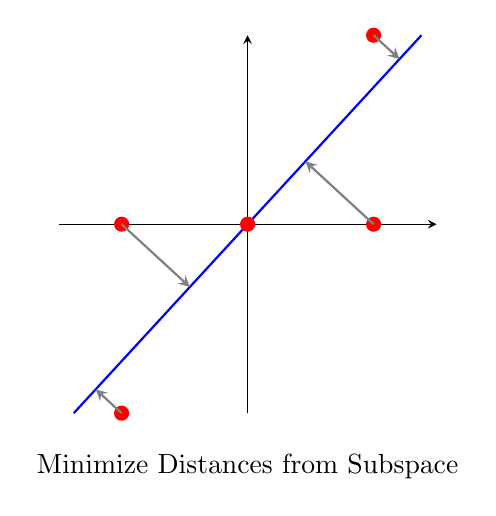
\begin{tikzpicture}[scale=0.8]
      \draw[thin,->] (-3,0) -- (3,0);
      \draw[thin,->] (0,-3) -- (0,3);
      \draw[thick,blue] (-3*0.92,-3) -- (3*0.92, 3);
      \fill[color=red] (0,0) circle (0.12);
      \fill[color=red] (2,0) circle (0.12);
      \fill[color=red] (2,3) circle (0.12);
      \fill[color=red] (-2,0) circle (0.12);
      \fill[color=red] (-2,-3) circle (0.12);
      \draw[thick, ->,black!50] (2,0) -- (0.997*0.92,0.997);
      \draw[thick, ->,black!50] (2,3) -- (2.621*0.92,2.621);
      \draw[thick, ->,black!50] (-2,0) -- (-0.997*0.92,-0.997);
      \draw[thick, ->,black!50] (-2,-3) -- (-2.621*0.92,-2.621);
      \path (0,-3.5) node[below] {Minimize Distances from Subspace};
      %\path[black!70] (2,-2) node {\begin{tabular}{c}minimize\\distances\\perpendicular\\to subspace\end{tabular}};
    \end{tikzpicture}
  \end{equation*}

  \begin{center}
    \geogebra{hp7wxjegkk}{630}{631}
  \end{center}


\end{document}